\documentclass[xcolor=dvipsnames]{beamer}
\usepackage{subfig}
\usepackage{wrapfig}
\usetheme{Rochester}  %% Themenwahl
\usecolortheme[named=RoyalBlue]{structure}
\usebackgroundtemplate{
	\centering
	\includegraphics[width=\paperwidth,height=\paperheight]{images/light-speed}
} 

 \addtobeamertemplate{block begin}{\pgfsetfillopacity{0.5}}{\pgfsetfillopacity{1}}
 \addtobeamertemplate{block alerted begin}{\pgfsetfillopacity{0.5}}{\pgfsetfillopacity{1}}
 \addtobeamertemplate{block example begin}{\pgfsetfillopacity{0.5}}{\pgfsetfillopacity{1}}

\setbeamertemplate{navigation symbols}{}

\title{Solve'n Slide}
\subtitle{Final Presentation}
\author{Hanieh Arjomand-Fard\\Kevin Sawischa\\Markus Ansorge\\Stefan Aicher}
\date{24. July 2017}

\begin{document}
	\maketitle
	
	\begin{frame}
		\frametitle{Proposal}
		\vspace{-1cm}
		\begin{figure}[H]
			\centering
			\begin{tabular}{cc}
				\subfloat{\includegraphics[height=4.5cm]{images/bigIdeaBullseye}}&
				\subfloat{\includegraphics[height=4.5cm]{images/Part2DecreaseCharge}}
			\end{tabular}
		\end{figure}
		\vspace{-0.2cm}
		\begin{figure}[ht]
			\includegraphics[scale=0.35]{images/LevelWithManipulation}
		\end{figure}
	\end{frame}
	
	\begin{frame}
		\frametitle{Game Prototype}
		\begin{columns}[T]
			\begin{column}{0.5\textwidth}
				\vspace{1cm}
				\begin{itemize}
					\setlength\itemsep{1em}
					\item Sandbox as best approach
					\item Level design not obvious
					\item But also not evident as sliding can't be simulated
					\item Only good for very rough surfaces
					\item All in all helpful to create levels
				\end{itemize}
			\end{column}
			\hspace{-1cm}
			\begin{column}{0.5\textwidth}
				\begin{figure}[ht]
					\includegraphics[scale=0.5]{images/final/Bild1}
				\end{figure}
			\end{column}
		\end{columns}
	\end{frame}
	
	\begin{frame}
		\frametitle{Interim}
		\begin{itemize}
			\item Mostly finished low target (Basic UI, movement, terrain manipulation, turret, levels)
			\item Started with desirable target (basic models without animations)
		\end{itemize}

		\begin{figure}[H]
			\centering
			\begin{tabular}{cc}
				\subfloat{\includegraphics[height=4.5cm]{images/interim/screenshot}}&
				\subfloat{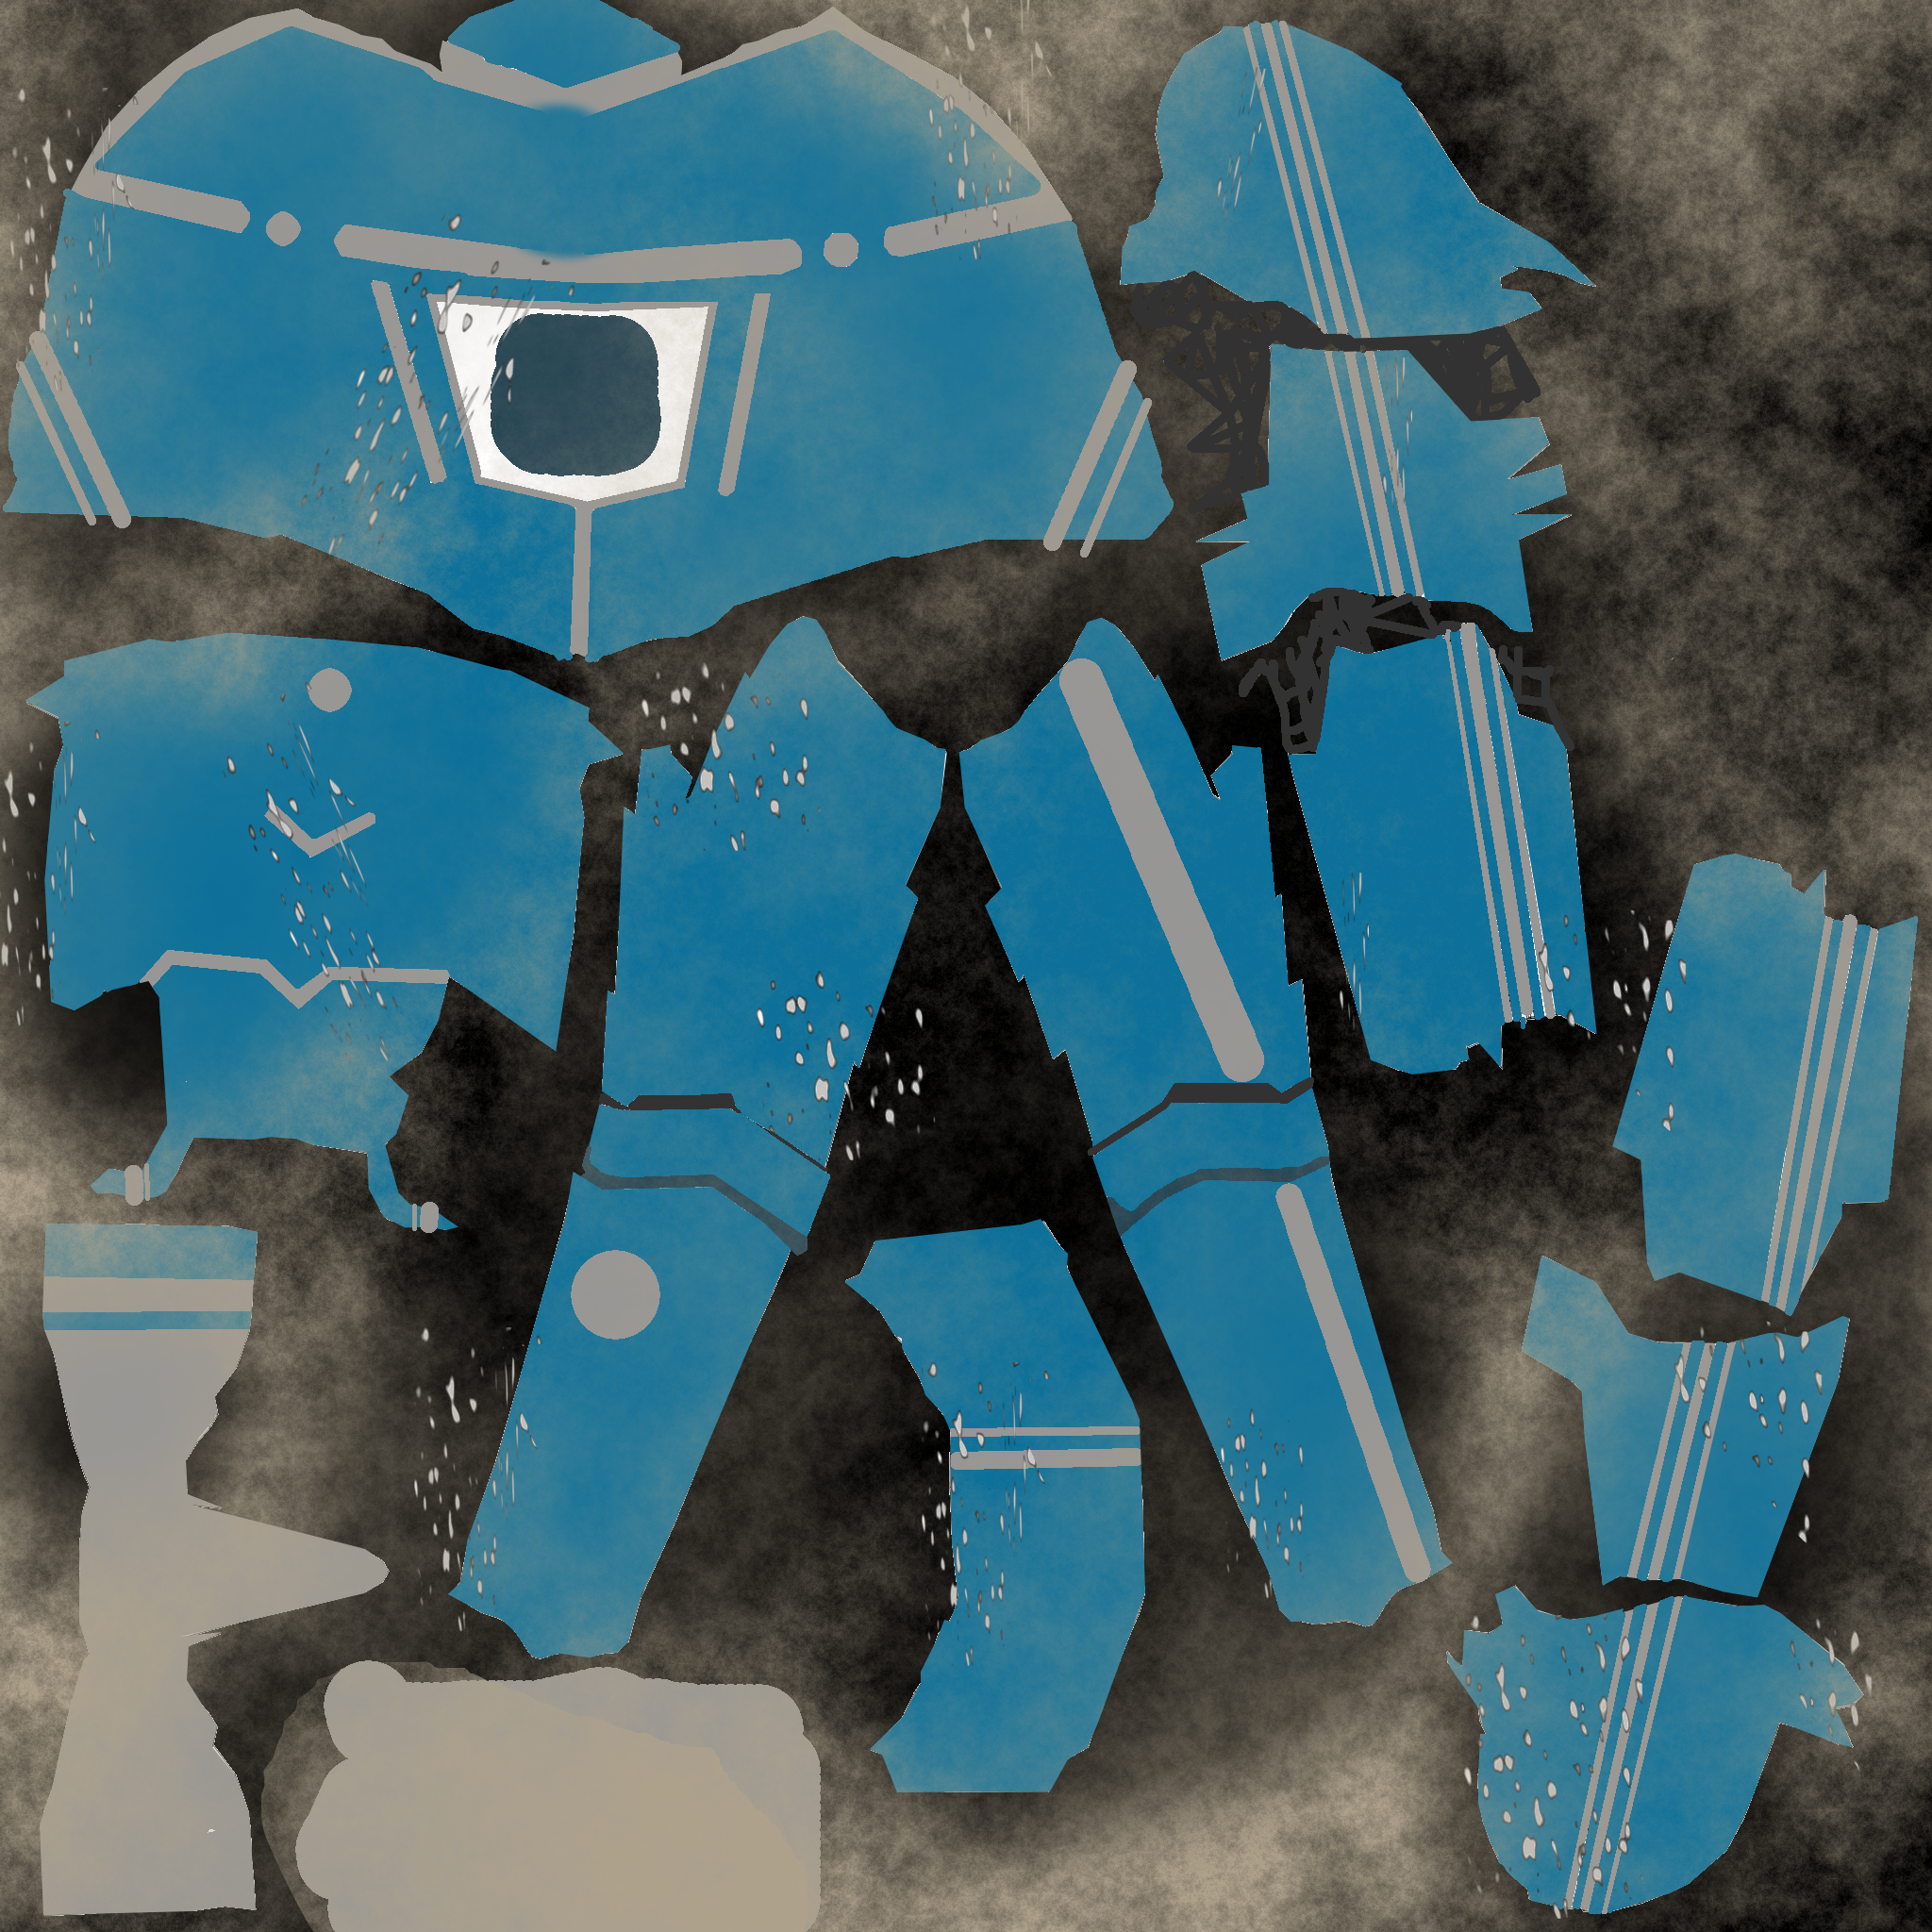
\includegraphics[height=4.5cm]{images/interim/character}}
			\end{tabular}
		\end{figure}
	\end{frame}
	
	\begin{frame}
		\frametitle{Alpha}
		\begin{itemize}
			\item Completed desirable target (proper terrain manipulation, main menu, UI, particle effects, animations, miscellaneous)
		\end{itemize}
		\vspace{-0.5cm}
		\begin{figure}[H]
			\centering
			\begin{tabular}{cc}
				\subfloat{\includegraphics[height=3.5cm]{images/alpha/mainMenu}}&
				\subfloat{\includegraphics[height=3.5cm]{images/alpha/boneWeights}}
			\end{tabular}
		\end{figure}
		\vspace{-0.5cm}
		\begin{figure}[H]
			\centering
			\begin{tabular}{cc}
				\subfloat{\includegraphics[height=2cm]{images/alpha/rocketTrailFireFX}}&
				\subfloat{\includegraphics[height=2cm]{images/alpha/chargeIcon}}
			\end{tabular}
		\end{figure}
	\end{frame}
	
	\begin{frame}
		\frametitle{Playtesting}
		\begin{itemize}
			\item Live testing via Skype
			\item Another point of view
			\item Found many bugs
			\item "Game too hard"
			\item Wishes and hints to improve the game
			\begin{itemize}
				\item More casual
				\item Fun oriented
			\end{itemize}
			\item Theoretically more playtesting instead of one time would be better
			\begin{itemize}
				\item To go in a better direction during development
			\end{itemize}
		\end{itemize}
	\end{frame}
	
	\begin{frame}
		\frametitle{Changes}
		\begin{figure}[ht]
			\includegraphics[scale=0.4]{images/final/mainMenu1}
		\end{figure}
		\vspace{-0.5cm}
		\begin{figure}[H]
			\centering
			\begin{tabular}{cc}
				\subfloat{\includegraphics[height=2cm]{images/final/movingClouds1Border}}&
				\subfloat{\includegraphics[height=2cm]{images/final/movingClouds2Border}}
			\end{tabular}
		\end{figure}
	\end{frame}
	
	\begin{frame}
		\frametitle{Changes}
		\hspace*{-0.4cm}
		\includegraphics[scale=0.34]{images/final/effectsCombined}
	\end{frame}
	
	\begin{frame}
		\frametitle{Conclusion}
		\begin{itemize}
			\setlength\itemsep{1em}
			\item Game is a success
			\item Learned a lot
			\item Good experience with the course
			\item Theme was alright
			\item Wished for more playtesting
		\end{itemize}
	\end{frame}
	
	\begin{frame}
		\frametitle{Demo}
		\centering
		\Huge
		Time for a live demo!
	\end{frame}
	
\end{document}